\section{TinyDAS}

In this section, we introduce TinyDAS, a Python program aimed at training autoencoder models and detecting anomalies in \acrshort{das} data. In this program, we use a combination of Tinygrad and Pytorch for training and testing our models. For the anomaly detection module, we utilize a combination of sklearn and Seaborn to evaluate our models.

\subsection{Tools}

Python is a dynamically typed, weak language famously known for it's \textit{easy-to-learn} syntax. Created by Guido Van Rossum in the late 80-s \cite{python}, Python has slowly emerged as one of the fastest growing programming languages ever created \cite{srinath2017python}. 

Virtually all of the larger libraries for data science and \acrlong{ml} have bindings to \gls{python}, or are written in Python from scratch. Some examples include \texttt{Pandas}, \texttt{NumPy}, \texttt{SciKit Learn}, \texttt{Pytorch} and \texttt{TensorFlow}. Many of these rely on code written in C or C++ to be fast, sincc

\subsubsection{Pytorch}

\subsubsection{Tinygrad}




\subsection{Overview}

An overview of how TinyDAS works is shown in the figure below \ref{fig:dataflow}.

\begin{figure}[h]
    \centering
    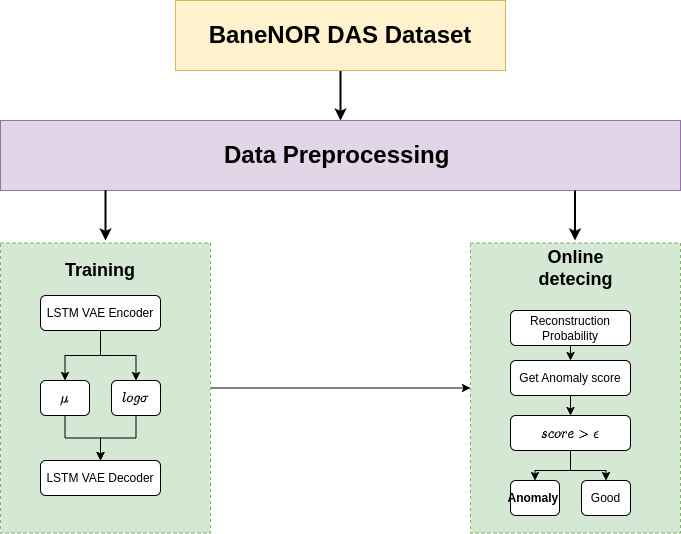
\includegraphics[scale=0.5]{figures/methodflow.png}
    \caption{Dataflow}
    \label{fig:dataflow}
\end{figure}

\subsection{Dataset}

For this project, we will be using the FORESEE dataset 
 as part of the PubDAS collection. \cite{spica2023pubdas}

\subsection{Usage}




\subsubsection{File format}

PubDAS consist of 8 datasets stored in 3 different file formats. These 3 are \texttt{TDMS}, \texttt{HDF5} and \texttt{SEG-Y}. 
The FORESEE

\subsubsection{Metadata}

\begin{table}[h]
    \small
    \centering
    \begin{tabular}{|l|l|}
    \toprule
    \multicolumn{1}{|c|}{\textbf{Name}} & \multicolumn{1}{c|}{\textbf{Value}} \\ \hline
    IU                                  & Silixa iDAS-v2                      \\ \hline
    Time Span                           & 365 days                            \\ \hline
    Format                              & HDF5                                \\ \hline
    Sample rate (Hz)                    & 125 (From 500)                      \\ \hline
    Volume (GB)                         & 29,338                              \\ \hline
    Gauge length (m)                    & 10                                  \\ \hline
    Cable Length (m)                    & 4900                                \\ \hline
    Channel spacing (m)                 & 2                                   \\ \hline
    File duration (s)                   & 60                                  \\ \hline
    Name format                         & FORESEE\_UTC\_YYYYMMDD\_HHMMSS:MMM.hdf5 \\ 
    \bottomrule
    \end{tabular}
    \caption{Metadata of the Foresee dataset}
    \label{tab:foresee_meta}
\end{table}

\subsubsection{Pre processing}

As opposed to the dataset from BaneNOR, the FORESEE dataset is already preprocessed. A lowpass filter is applied on the data. TBD ... \\

When first downloading these data, they're stored in 10-minute files, resulting in quite large files as shown below:

\begin{align*}
\text{Size} &= 10 \times 60 \times 125 \times 2137 \times 4 \\
&= 600 \times 125 \times 2137 \times 4 \\
&= 641,100,000 \text{ bytes} \\
&\approx 641.1 \text{ MB} \\
&\approx 0.6411 \text{ GB}
\end{align*}

where:
\begin{itemize}
    \item 10 minutes is the duration of each file
    \item 60 seconds per minute
    \item 125\si{\hertz} is the sampling rate
    \item 2137 is the number of channels
    \item 4 bytes per sample (Float32)
\end{itemize}

Most consumer grade \acrshort{gpu}s can only store about 8-16gb of data in VRAM, thus meaning the batches of data we can store is not that big. Additionally, not only does the \acrshort{gpu}s have to store data, but also the weights and biases of the model, as well as losses and more. Motivated by this, we decide to split the files to last 5 seconds compared to 10 minutes. \\ 

We start of by looking at the file names and removing the prefix \textbf{FORESEE\_UTC\_}, since we're only working with one dataset at the time. Furthermore, in parallel fashion, we split each of the files in smaller ones, calculating new filenames based on the beginning timestamp. Now, each \acrshort{hdf5} file store a $625*2137$ matrix of \acrshort{das} data, successfully reducing the memory usage. 
These data are originally stored as \texttt{Float32}, but will be casted as \texttt{Float16} for faster training as we will see later on. In total, more than 25 000 files from the month of april 2020 is gathered to train our model on. 
RESULT: SPEAK ABOUT 5 SECONDS FOR LIVE ENVIRONMENT.
TODO: Inference data from 15042019!

TinyDAS is a program we've created to easily be able to train, and test different types of autoencoder models for anomaly detection. The main ideas behind creating this program are as follows:

\begin{enumerate}
    \item New autoencoder models are easy to add
    \item Easy to tune configurations
    \item Scalable from single core computer to distributed systems.
    \item The program is not tied to any particular hardware accelerator architecture
    \item Support for half precision training
    \item Support for transfer learning and early stopping
    \item Testing of autoencoders should be easy to add
\end{enumerate}

Based on these conditions, our choice of framework was tinygrad \ref{back:tinygrad}, mainly since the framework is designed to be accelerator-independent.

\subsection{\acrshort{api} design}

\subsubsection{Datasets and Dataloaders}

For easy swap out between datasets, we introduce two classes, \texttt{Dataset} and \texttt{DataLoader}. The former handles information about the dataset to be trained on, as well as logic for loading a single file from a \acrshort{hdf5} file, or whatever other format might be sent in later on. The latter one handles loading of batches in parallel, loading $n$ samples into the model.

\subsubsection{Autoencoder Base Class}

\lstinline{BaseAE} is the abstract class which all the different models inherit from. The \lstinline{criterion} method is the main method to use when using a model. It runs the \lstinline{__call__} method, apply the loss function of choice, and stores in a dictionary in case we'd like to store multiple losses. We define the class as follows:

\lstinputlisting[language=Python, label={lst:baseae}, caption=Base Autoencoder class]{code/baseae.py}

As we see in the listing above \ref{lst:baseae}, we also provide method in here for prediction. 

\subsubsection{Early Stopping}

Even though the model loss ideally should decrease to eventually reach zero almost immediately, this is never the case. Overfitting is when the loss starts increasing, never to return to its best value. To avoid spending time and resources on unnecessary training, we implement a useful mechanism called early stopping, which is described as follows:


\begin{align*}
&\text{Stop at epoch } T \text{ if:} \\
&\forall i \in \{T-p+1, ..., T\}: L_v(i) > L_v^* - \epsilon \\
&\text{where } L_v^* = \min_{j=1}^{T} L_v(j) \\
\\
&\text{Given:} \\
&L_v(t) \text{ is the validation loss at epoch } t \\
&p \text{ is the patience (number of epochs to wait)} \\
&\epsilon \text{ is a small threshold for improvement}
\end{align*}

\subsubsection{Trainer}

The Trainer class serves as the core component of our program. As demonstrated in listing \ref{fig:lstmcell}, it integrates a model, dataloader, and optimizer to execute the training process. Additionally, it handles early stopping, storing history of losses and saving the best model for further use.

\subsubsection{Hyperparameters and configurations}

To set hyperparameters 

\subsection{Evaluation}

We will be splitting the evaluation of \texttt{TinyDAS} in two sections. The first section will focus more on overall model training. Here is a list of points to be evaluated: 

\begin{itemize}
    \item \textbf{Experiment 1}: Median training time and model sizes
    \item \textbf{Experiment 2}: Losses
    \item \textbf{Experiment 3}: Reconstruction Capabilities
\end{itemize}

The section will revolve around anomaly detection based on the different architectures.

\begin{itemize}
    \item \textbf{Experiment 1}: Anomaly Detection Accuracy
    \item \textbf{Experiment 2}: Confusion Matrix and Metrics
\end{itemize}

